\subsection{Représentation des connaissances}
\label{subsection_representation_co}
	Les connaissances seront représentées en logique du première ordre. D'une part le plateau sera représenter comme un ensemble de faits et d'autres part les \og formes \fg{} seront représentées par des règles dont l'hypothèse représente la sous structure à reconnaître et la conclusion représente un identifiant de cette forme.
	
	\subsubsection{Vocabulaire} 
	\begin{itemize}
		\item isMine(x)
  	\item isOpp(x)
  	\item isEmpty(x)
  	\item isEdge(x)
  	\item isCorner(x)
  	\item near(x,y)
  	\item aligned(x,y,z)
	\end{itemize}

\label{specs_voc_fol}

\subsection{Le package FOL}
\label{subsection_fol}

Le package \package{FOL} pour \og First Order Logic \fg{} contient l'ensemble des classes représentant des informations en logique du première ordre.

\begin{itemize}
  \item \textbf{\class{\gls{Cbs}}} : \og Complete Board State \fg{}, c'est la version logique du premier ordre de \class{\gls{BoardMatrix}} définie section \vref{game_logic_shared}.
  
  \item \textbf{\class{\gls{Rpbs}}} : \og Relevant Partial Board State \fg{}, la classe qui décrit la configuration d'une sous-partie pertinente d'un plateau comme une règle logique. Elle correspond aux \og formes \fg{} extraites par le module de raisonnement qui doivent être reconnues dans les \class{\gls{CompleteBoardState}}.
  
   \item \textbf{\class{\gls{Option_FOL}}} : C'est la version logique de la classe \class{Option}.
   
   \item \textbf{\class{\gls{Choices_FOL}}} : Elle est la version convertie par l'analyseur de Choices (même structure, attributs décrits par des formules logiques) avec, en addition, une liste de formes pertinentes associée à chaque plateau du paquet.
\end{itemize}


\subsection{Spécifications des classes Cbs et Rpbs}
\label{subsection_cbs_rpbs}

\begin{figure}[H] 
\centering
    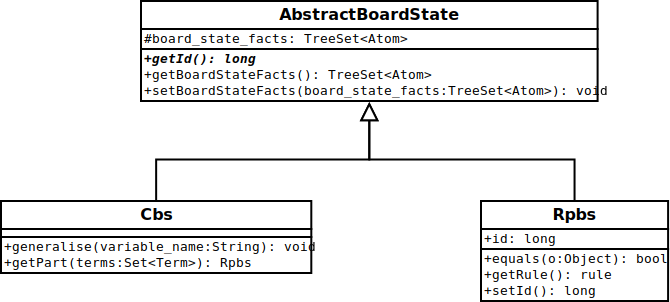
\includegraphics[width=\textwidth]{files/class_diagram/rpbs_cbs} 
\caption{Diagramme de classe des Cbs et Rpbs.} 
\label{img_diag_class_board_state}
\end{figure}

Les classes \class{\gls{Cbs}} et \class{\gls{Rpbs}} représente respectivement un plateau et une sous configuration d'un plateau dans le format logique décrit en \vref{subsection_representation_co}. 

\subsection{Misc.}
\begin{itemize}
  \item \textbf {\texttt{\gls{Choices} (environnement)}} : Cette classe est un pacquet qui représente un plateau courant, un coup et l'ensemble des plateaux résultants de ce coup, où chaque plateau est une instance de la classe \texttt{\gls{BoardMatrix}} définie ci-après. Elle appartient à la bibliothèque \texttt{\gls{game_logic}} de l'environnement.
  \item \textbf {\texttt{\gls{BoardMatrix}(environnement)}} : C'est la classe de base qui représente un plateau en forme d'une matrice. 
  \end{itemize}
